% MODULE 9: DELAYS, CO-DESIGN, AND NONLINEAR CHECKS. Panel box (reference px): x 764-1148, y 796.5-1129.5, title bar to y 822.5.
% Design v2: A commutator law (HeroBox, EXACT), B delay root locus (plot), C workflow strip (cards), D nonlinear event dots, red NoteBox.
\begin{scope}
  % ---------------------------------------------------------------- A: unequal latencies mix graph modes (EXACT)
  % source: experiments/theory_collective_damping_20261003/THEORY.tex eq:freqcomm (EXACT_IDENTITY) and CLOSURE_SYMBOLIC_CHECKS.json
  \SubHead{A}{Unequal latencies mix graph modes}{775}{833}
  \ProvedTag{1112}{833}{EXACT}
  \HeroBox{775}{843}{1139}{886}
  \node[anchor=west,inner sep=0pt,text=PNavy] at (785,851.5) {\fontsize{21pt}{23pt}\selectfont $E_\tau(s)=\mathrm{diag}\,e^{-s\tau_i},\quad [L,K(L)E_\tau]=K(L)\,[L,E_\tau]$};
  \node[anchor=west,inner sep=0pt,text=PNavy] at (785,869.5) {\fontsize{28pt}{30pt}\selectfont $\|[L,E_\tau(j\Omega)]\|_F^2=8\!\!\sum_{ij\in\mathcal E}\!w_{ij}^2\sin^2\!\Big(\tfrac{\Omega(\tau_i-\tau_j)}{2}\Big)$};
  \node[anchor=east,inner sep=0pt,text=PGreen,font=\FiraSemi\fontsize{17.5pt}{17.5pt}\selectfont] at (1136,879.5) {zero only if $\tau_i=\tau_j$ on every edge};

  % ---------------------------------------------------------------- C: workflow strip (left column)
  \SubHead{C}{Co-design loop}{775}{898}
  % steps: y centre / label (two lines) / kind (0 normal, 1 emphasised)
  \draw[PGold,line width=1.8pt,line cap=round] (788,918) -- (788,1117);
  \foreach \y/\l/\k in {918/{Choose the\\portfolio}/0, 949.5/{Equilibrium and\\full spectrum}/0, 981/{Diagnose closure\\$Q$ and $D_H$}/0, 1012.5/{Choose the\\radius $n$}/0,
      1044/{Gain map and\\predictor}/0, 1075.5/{FULL-SPECTRUM\\corrector}/1, 1107/{Nonlinear\\events}/0}{
    \ifnum\k=1
      \fill[PGreen,rounded corners=3pt] (776,\y-14.5) rectangle (925,\y+14.5);
      \fill[PGold] (776,\y-14.5) rectangle (779.5,\y+14.5);
    \else
      \CardBox{776}{\y-14.5}{925}{\y+14.5}
    \fi}
  \foreach \y in {933.5,965,996.5,1028,1059.5,1091}{\fill[PGold] (783,\y-3) -- (793,\y-3) -- (788,\y+3) -- cycle;}
  \foreach \y/\n in {918/1, 949.5/2, 981/3, 1012.5/4, 1044/5, 1075.5/6, 1107/7}{\StepNumber{801}{\y}{\n}}
  % the step discs sit on the connector; labels start at x 815
  \foreach \y/\l in {918/{Choose the\\portfolio}, 949.5/{Equilibrium and\\full spectrum}, 981/{Diagnose closure\\$Q$ and $D_H$}, 1012.5/{Choose the\\radius $n$}, 1044/{Gain map and\\predictor}, 1107/{Nonlinear\\events}}{
    \node[anchor=west,inner sep=0pt,text=PText,align=left,font=\FiraSemi\fontsize{18.5pt}{20pt}\selectfont] at (815,\y) {\l};}
  \node[anchor=west,inner sep=0pt,text=white,align=left,font=\FiraBold\fontsize{18.5pt}{20pt}\selectfont] at (815,1075.5) {FULL-SPECTRUM\\corrector};

  % ---------------------------------------------------------------- B: delay root locus (right column)
  \SubHead{B}{Delay root locus}{935}{898}
  \ObservedTag{1103}{898}{NUMERICAL}
  % source: research/feedback_cycle_fullmodel_20261005/derived/TABLE_D01_delay_continuation.csv (PLL family, 9 branches) and TABLE_D01b_delay_crossings.csv (41.57 ms = R0 margin crossing)
  \node[anchor=north west,inner sep=0pt] at (933,907) {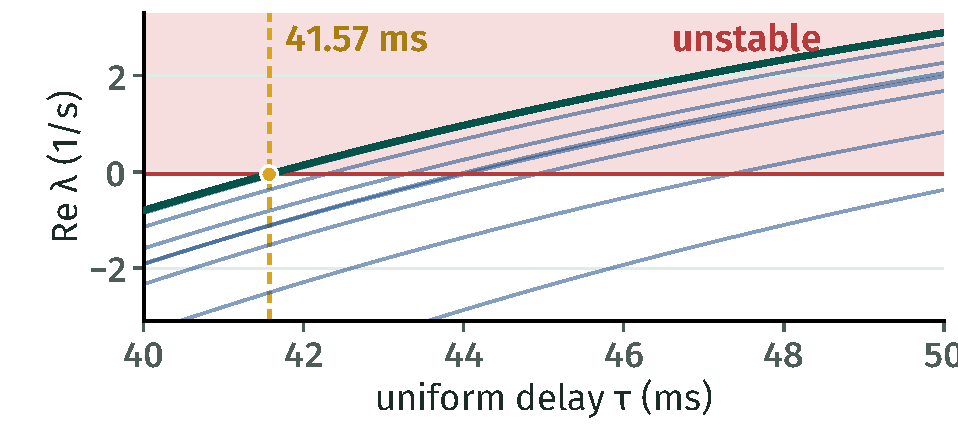
\includegraphics[width=206\PX,height=92\PY]{figures/module9/m9_delay_locus.pdf}};
  \node[anchor=north west,inner sep=0pt,text=PMuted,font=\FiraMed\fontsize{17pt}{17pt}\selectfont] at (935,1000.5) {Full IEEE-39, exact delay; margin $-0.05\,\mathrm{s^{-1}}$};

  % ---------------------------------------------------------------- D: nonlinear checks as event dots
  \SubHead{D}{Five frozen nonlinear events}{935}{1019}
  % source: research/nhop_ieee39_20261006/derived/E6_events.csv (events_passed, failures) and research/feedback_cycle_fullmodel_20261005/derived/TABLE12_nonlinear_events.csv (EV_uniform_kp, 44 ms: 5 of 5 pass)
  \foreach \cx/\h in {1003/$n{=}0$, 1039/$n{=}1$, 1075/$n{=}3$}{
    \node[inner sep=0pt,text=PMuted,font=\FiraSemi\fontsize{17pt}{17pt}\selectfont] at (\cx,1031) {\h};}
  \foreach \y/\lab in {1044/{48\,ms}, 1058/{52\,ms}, 1072/{44\,ms, 90\,\%}, 1086/{44\,ms, $K_p\,{-}14\,\%$}}{
    \node[anchor=west,inner sep=0pt,text=PText,font=\FiraMed\fontsize{17pt}{17pt}\selectfont] at (935,\y) {\lab};}
  % dots: pass = teal, fail = red; x0 = first dot of the group, y row, pattern of five 1/0
  \newcommand{\DotsGroup}[3]{\foreach \p [count=\i from 0] in {#3}{\ifnum\p=1 \fill[PTeal] ({#1+\i*6.6},#2) circle (2.7);\else \fill[PRed] ({#1+\i*6.6},#2) circle (2.7);\fi}}
  \DotsGroup{990}{1044}{1,1,1,1,1}   \DotsGroup{1026}{1044}{1,1,1,1,1}
  \DotsGroup{990}{1058}{1,0,1,1,1}   \DotsGroup{1026}{1058}{1,1,1,1,1}   \DotsGroup{1062}{1058}{0,0,0,0,0}
  \DotsGroup{990}{1072}{0,0,0,0,0}   \DotsGroup{1026}{1072}{0,0,0,0,0}
  \DotsGroup{1049}{1086}{1,1,1,1,1}
  \node[anchor=west,inner sep=0pt,text=PMuted,font=\FiraMed\fontsize{16pt}{16pt}\selectfont] at (1091,1072) {$|\Delta f|>0.5$\,Hz};
  \node[anchor=west,inner sep=0pt,text=PTeal,font=\FiraSemi\fontsize{16pt}{16pt}\selectfont] at (1091,1086) {5/5};

  % ---------------------------------------------------------------- red note: necessary, not sufficient
  \NoteBox{933}{1097}{1139}{1128}{PRed}
  \node[anchor=west,inner sep=0pt,text=PRed,font=\FiraBold\fontsize{20pt}{20pt}\selectfont] at (942,1106) {Spectral margin is necessary,};
  \node[anchor=west,inner sep=0pt,text=PRed,font=\FiraBold\fontsize{20pt}{20pt}\selectfont] at (942,1118.5) {not sufficient.};
\end{scope}
